\section{Introduction}
\label{sec:bcoolintro}
This chapter presents \bcool, a dedicated (meta)language to explicitly capture the knowledge about system integration. With \bcool, an integrator can deal with the complexity of the coordination of heterogeneous behavioral models by capturing coordination patterns at the language level. To do so, he defines operators that specify how the \dse of different language behavioral interfaces are combined and interact. Once specified in \bcool, such specification can be shared thus allowing reusing and tuning of coordination patterns. Also, system designers can use it to generate an explicit coordination model when specific models are used.    
	
In this chapter, we illustrate the use of \bcool through a (simple) running example: the coordination of the model of a coffee machine. To build the model, we base on two languages: a state-based language named Timed Finite State Machine (TFSM) and an action-based language named Activity. We use the TFSM to model the control-flow aspects and the Activity to model the data-flow aspects. The model of the coffee machine is thus heterogeneous. We propose to automate the coordination of the models of the running example by relying on a \bcool operator between these languages.

This chapter begins by presenting the running example and the languages together with its behavioral interface.  Then, we continue the chapter by presenting the abstract syntax and the semantics of \bcool. To illustrate the use \bcool, we rely on the running example. Then, we present the implementation of \bcool into the GEMOC studio. To finish the chapter, we evaluate and compare our approach with coordination languages and frameworks and we conclude.

%\begin{figure}
%	\begin{center}
%		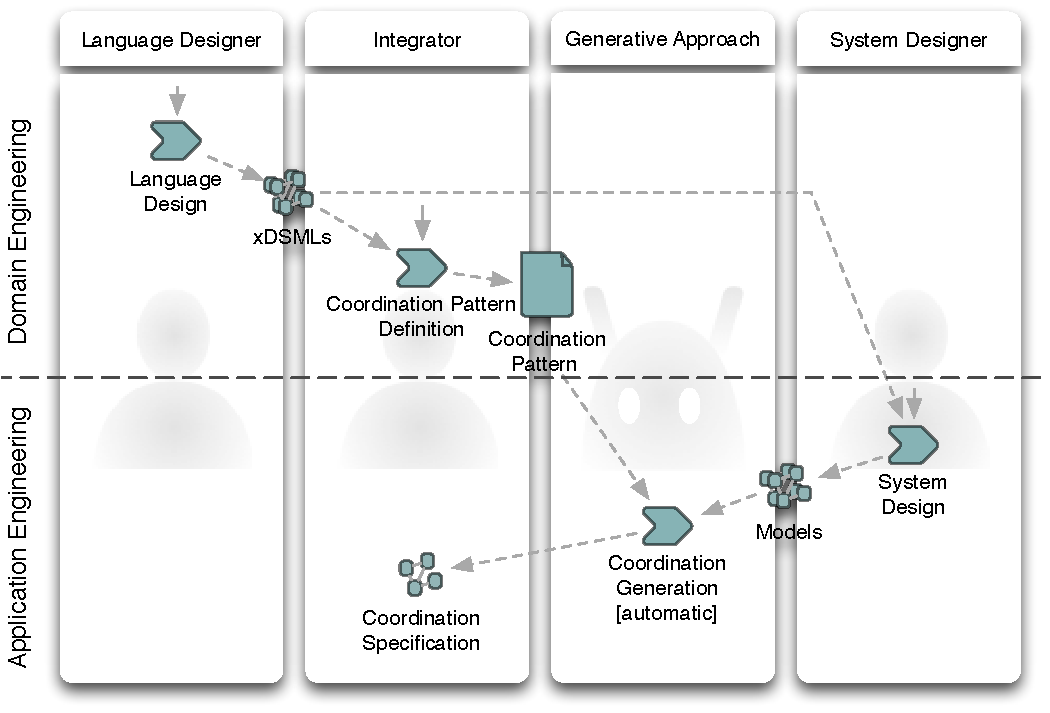
\includegraphics[width=.6\textwidth]{bcool/figs/process}
%		\caption{The Proposed Workflow}
%		\label{fig:proposedworkflow}
%	\end{center}
%\end{figure}

%The running example helps us to illustrate the different tasks in the development of heterogeneous systems:
%	\begin{enumerate}
%		\item Designing of the languages.
%		\item Integration of the languages. 
%		\item Building of the models. 
%		\item Coordination of the models. 
%	\end{enumerate}
%In this context, \bcool deal with the task number two and four. 